\section{Avant d'implémenter}
Avant de réaliser la simulation il faut savoir que 
la mise en place des cellules dans la simulation relève de deux choses : 
\begin{itemize}
	\item La mise en place d'une classe Gérant de simulation
	\item La mise en place d'une classe Cellule
\end{itemize}

La cellule se contente d'exister, de mourrir, de muter, d'avoir une couleur, une position. Le Gérant lui, est l'environnement de la cellule, il contient toutes les cellules d'une simulation, et c'est lui qui les traites. Pour afficher les cellules, on demande au gérant de le faire. Pour ajouter une cellule à une position, on demande au gérant, quand une cellule veut se diviser, elle demande au gérant, parce que lui sait si elle peut se diviser, ou s'il n'y a plus d'espace libre autour d'elle.

Le code complexe se trouvera donc dans la classe Gérant. Elle est avec le système de boucle, le centre du code, autour duquel le reste s'articule.

\section{Cellule}

Avant de représenter une cellule il faut se demander ce que l'on va représenter. Nous avons choisi dans un premier temps de nous simplifier la tache en la considérant comme un objet simple qui a les membres suivants : 
\begin{itemize}
	\item un nombre de cycles
	\item un nombre de mutations
	\item un nombre 
\end{itemize}

Bien entendu, la classe Cellule hérite de Rectangle, vu qu'elle sera dessinée à l'écran.

Le code complexe des cellules se trouvera en réalité dans le gérant, simplement car il a les informations sur les autres cellules voisines, mais nous en parlerons tout de même dans cette section.

\subsection{Division}

La fonction la plus importante des cellules est la division. C'est aussi la fonction qui pose le plus de problèmes purement algorithmiques. Résumons :
\begin{itemize}
  \item La division doit se produire une fois toutes les $N$ minutes en fonction des cellules
  \item La division crée une cellule mère et une cellule fille\footnote{Contrairement à ce que l'on pensait encore récemment, les cellules ne sont pas identiques, et une cellule mère «~vieillit~» au fur et à mesure des divisions}.
  \item La direction de la division n'est pas déterminée
\end{itemize}

  Donc il faudra créer une nouvelle cellule toutes les $N$ minutes, qui aura les mêmes caractéristiques que sa mère, sauf l'age, et à une position contiguë à la cellule mère indéterminée.
  
  Pour pouvoir créer une cellule quelque part, il faut vérifier que l'espace est vide. On a donc appliqué la méthode suivante : \begin{itemize} \item Si la case $N$ est vide alors on divise sinon continuer 
            \item Si une autre case $N'$ est vide alors on divise sinon continuer
            \item etc … 
            \end{itemize}
  Pour plus de réalisme, nous avons testé différentes configurations : 
    \begin{figure}[H]
      \centering
      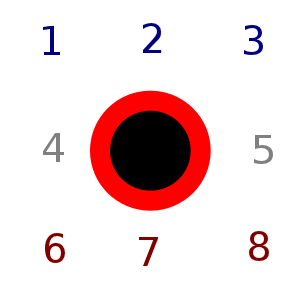
\includegraphics[width=15em]{Images/div_1.png}
      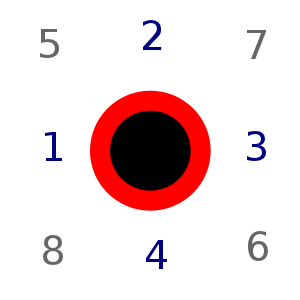
\includegraphics[width=15em]{Images/div_2.png}
      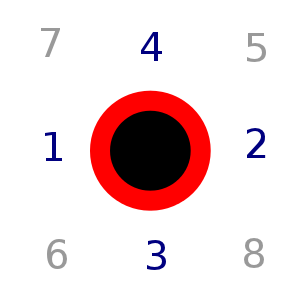
\includegraphics[width=15em]{Images/div_3.png}
      \caption{Schémas de l'ordre de vérification des cases}
    \end{figure}
  
  Une fois déterminé l'ordre de division, il faut prendre en compte un autre paramètre : lorsqu'il n'y a aucun espace possible, les cellules se «~poussent~» pour créer assez de place. Faute de temps, nous n'avons pas pu mettre en place une gestion de cette poussée dans les 6 directions, mais uniquement dans les 4 principales. Le code déplace toutes les cellules d'une case, et ensuite permet à la cellule de se diviser. Cette option créer un véritable tapis de cellules qui mélange tous les ages, du fait des déplacements. \\

\subsection{Couleur}
  Une deuxième chose, qui cette fois n'est pas gérée par le Gérant mais par l'Afficheur, et qui concerne directement les cellules : les codes de couleur. Nous avons choisi d'utiliser des codes de couleur pour signifier les différences entre les cellules selon le modèle suivant : 
    \begin{figure}[H]
      \centering
      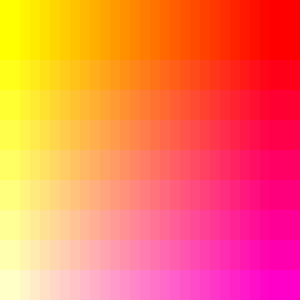
\includegraphics[width=20em]{Images/test.png}
      \caption{Dégradé des couleurs des cellules}
    \end{figure}
    
  La lecture de ce graphe est la suivante : On part du coin haut gauche pour la cellule normale. Plus on se déplace vers la droite, plus la cellule est vieille. Plus on descend, plus la cellule a subit des mutations.
  
  Malheureusement, il n'est parfois pas très lisible de combiner deux dégradés de couleur sur une seule cellule. Mais c'est le moyen qui est le plus lisible de tous, car il est indépendant de la taille des cellules.
  
\subsection{UV}
  Nous avons souvent parlé des UV, mais jamais nous n'avons implémenté de fonctions qui déterminaient les mutations et la mort des cellules quand les UV étaient activés. Grâce aux résultats des expériences et recherches, nous avons déterminé les taux de mutation en fonction du temps. Indépendamment nous avons déterminé le taux de mortalité aux UV. On peut les retrouver dans l'annexe \ref{DefLevures}.
  
  Ces taux sont des statistiques. Dans le programme, nous avons utilisé des nombres aléatoires avec des probabilités de sortie qui correspondaient aux statistiques. Nous avons toutefois du modifier un peu la courbe des mutations, pour la rendre plus facilement modélisable en une équation simple. Pour le taux de mortalité idem.
  
  Globalement les chiffres tirés correspondent, et la simulation fait ce qu'on attend d'elle. Mais vient le problème du fait que les UV sont très agressifs, et une heure d'exposition tue déjà un peu plus de la moitié des cellules de levures, alors qu'elles mettent environ deux heures à se diviser. Il en résulte un certain décalage, entre la rapidité de réaction aux UV et la vitesse de division, qui peut rendre étrange l'utilisation de la simulation.

\section{Gérant}
\subsection{Définition}
Nous devons définir les actions du gérant : 
\begin{itemize}
	\item Ajouter une cellule
	\item Tuer une cellule
	\item Diviser une cellule
	\item Dessiner les cellules
	\item Faire exécuter un cycle à toutes les cellules
\end{itemize}

\subsection{Stockage des cellules}

Devant ceci il nous faut un moyen de conserver les cellules efficacement.
Pour cela il faut connaître les structures de données décrites dans l'annexe \ref{DefTableaux} et \ref{DefListe}. Pour choisir entre une liste et un tableau\footnote{Il existe d'autres structures, mais pour cette simulation, liste et tableaux semblaient les plus pertinentes}, il faut avant tout connaître nos besoins. Au vu des actions définies plus haut voici les actions par ordre d'occurence à l'exécution : 
\begin{enumerate}
	\item Parcourir 
	\item Supprimer
	\item Ajouter
\end{enumerate}

Au vu des annexes \ref{DefTableaux} et \ref{DefListe}, le tableau semple beaucoup plus adapté, étant donné qu'il ne demande qu'un temps constant pour lire une valeur (cf \ref{Complexite}).

La conservation n'a rien à voir avec l'affichage, puisque toute Cellule a une position sur l'écran, indépendante de sa position dans le tableau.

Néanmoins, nous avons décidé pour plus de simplicité, de gérer aussi l'affichage des cellules sous la forme de grille. Donc, la position d'une cellule dépendra de sa case. Ceci n'est pas obligatoire, mais les points suivants défendent cette idée : 
\begin{itemize}
	\item Gérer les cellules «~librement~» induit une gestion des collisions, chose complexe et coûteuse en rapidité quand elle n'est pas optimisée
	\item Gérer les cellules en grille permet de mieux contrôler des divisions, et permet d'effectuer plus facilement une grille de comptage que des cellules libres 
	\item Gérer les cellules en grille permet de ne JAMAIS redimensionner le tableau, donc 
	toutes les opérations sont à complexité constante.
\end{itemize}

Nous avons donc réaliser la conservation des cellules dans un tableau à deux entrées, lignes et colones. En réalité, c'est un tableau de tableaux de cellules\footnote{Un tableau est une suite d'élément, sur une seule «~ligne~»}. Ce qui revient à un tableau à double entrée. On accède donc à une cellule en faisant : Gérant.recupCell (colone,ligne).

Les cases seront soit vide, soit avec une cellule. Dans le code, il faudra donc bien penser à toujours vérifier que la case contient une cellule avant de faire une action, ce qui cause malheureusement beaucoup de soucis qui sont difficiles à voir facilement.

Il en résulte que les cellules sont sous la forme de grille, ce qui laisse paraître une certaine rigidité dans la simulation. Néanmoins, quand les cellules sont petites, la grille aussi est petite, et le problème de «~cases~» se ressent moins.

\subsection{Manipuler les cellules}
	La gestion des cellules découle de l'utilisation d'un tableau. Le gérant doit néanmoins conserver d'autres variables, comme le nombre de cellules par exemple. Pour celui-ci, il va falloir mettre en place un compteur.
	Le principe est d'incrémenter le compteur de 1 à chaque création, et de le décrémenter de 1 à chaque destruction de cellule. On pourrait imaginer faire cela dans chaque fonction qui crée ou détruit une cellule. Mais cela ne serait sûrement pas judicieux. Au contraire, nous utiliserons les constructeurs et destructeurs\footnote{Voir l'annexe \ref{DefPOO} sur la POO} de la Classe Cellule pour incrémenter et décrémenter. Il en découle qu'il n'y a que 2 lignes de code à ajouter, aucun risque de bug, et un code plus lisible.
	
	De même, le gérant contient un code que l'on trouve souvent, avec juste quelques variantes : le parcours du tableau entier. En effet, pour afficher, pour exécuter, ou pour tout supprimer, on utilise une même boucle qui parcours le tableau, avec un code différent à l'intérieur. Au lieu d'utiliser Ctrl-C et Ctrl-V nos amis, nous allons introduire un concept magnifique de la programmation : le passage de fonction en argument. En paramètre d'une fonction on donne des variables, mais on peut aussi donner des fonctions ! De ce fait, nous pouvons créer une fonction «~parcourir (fn fonction);~» qui prend en paramètre la fonction à appliquer, et l'applique sur tous les éléments du tableau. Le code est plus modulaire, et plus facilement modifiable. Si la structure de stockage des cellules changeaient, il suffirait de changer le code dans «~parcourir~» plutôt que de changer toutes les fois où l'on a parcouru le tableau en entier. 


  Pour conclure nous avons maintenant un programme fonctionnel, dont nous avons expliqué le développement en prenant l'exemple du Menu comme objet périphérique de la simulation, et dont nous avons décrit les recherches de données qui ont permis de coder la simulation elle même.
  
  Le programme fait ce qu'on veut de lui, mais il reste quand même relativement simpliste, et en cela on est en mesure de se demander s'il répond bien aux attentes de départ.
